\chapter{物种形成与大进化}\label{ch:b2:speciation}

1982 年，在加拉帕戈斯群岛的一座小岛上，
一些大喙地雀从邻岛迁来并留了下来。
二十年间，它们与当地的中喙地雀
争夺两者都偏好的大\omterm{def:b2:angiosperm-reproduction:seed}{种子}；随后干旱来临，
大\omterm{def:b2:angiosperm-reproduction:seed}{种子}变少，喙较大的原住地雀——
即与新来者竞争最为直接的那些——因此饿死。
一代之内，原住地雀的喙明显变小，
与入侵者的喙拉开了距离。两个曾经相遇的物种被推开了。
本章讨论物种的形成：物种是什么，什么使它保持独立，
一个种群如何\omterm{def:b2:cell-differentiation:differentiation}{分化}为两个，
相遇时驱使种群分开的竞争，以及
从化石记录看到的长时间尺度——同一过程
重复一亿多次，形成了生命之树。

\section{什么是物种}

\begin{definition}[物种]\label{def:b2:speciation:species}
\index{物种概念}\index{生物学物种概念}\index{生殖隔离}
依据\emph{生物学物种概念}，物种是一组种群，
其成员彼此能够杂交并产生可育的后代，
且与其他此类群体\emph{生殖隔离}：统一物种的是\omterm{prop:b2:population-genetics:migration}{基因流}，
区分物种的是\omterm{prop:b2:population-genetics:migration}{基因流}的缺失。该概念适用于同一时间、同一地点的有性生物，
这也是生物学家遇到的大多数情形；
对无性谱系（只能依据相似性命名）、化石（无法杂交），
以及边界模糊的许多情形，该概念便不再适用——
例如跨物种杂交的栎树与柳树，
种间在圈养条件下相互杂交的鸭子，
以及环种（相邻种群环绕某一屏障相互杂交，
直到两端相遇而不能杂交）。
其他概念可以弥补这些不足：\emph{形态}物种（一群相似的类型）、
\emph{系统发生}物种（可被鉴别的最小谱系）、
\emph{生态}物种（占据自身\omterm{prop:b2:speciation:displacement}{生态位}的谱系）。
这些概念都没有错，
各自衡量的都是真实存在的东西；
物种形成则是它们逐渐趋于一致的过程。
\end{definition}

\begin{proposition}[隔离机制]\label{prop:b2:speciation:isolation}
\index{隔离机制}\index{合子前隔离}\index{合子后隔离}\index{霍尔丹法则}
两个种群之间的\omterm{prop:b2:population-genetics:migration}{基因流}，
会被发生在受精之前或之后的障碍所阻断。\emph{\omterm{prop:b2:speciation:isolation}{合子前隔离}}：种群
生活在不同的栖息地，或在不同季节繁殖
（时间隔离：两种青蛙在不同月份鸣叫）；它们不能识别彼此的求偶行为
（行为隔离：蟋蟀的鸣声、萤火虫的闪光信号、
鸭子的求偶舞蹈）；
它们的生殖器官或花的结构不相匹配（机械隔离）；它们的配子
不能融合（配子隔离：海胆的精子结合蛋白，
以及\cref{ch:b2:angiosperm-reproduction}中的$S$\omterm{def:b2:meiosis-heredity:vocabulary}{等位基因}）。
\emph{\omterm{prop:b2:speciation:isolation}{合子后隔离}}：杂种在胚胎期死亡，或存活但不育
（如骡子，以及两种\emph{Drosophila}物种的杂种），
或杂种可育但其自身的后代不育（杂种衰败）。
\emph{霍尔丹法则}：当杂种只有一种性别不育或不能存活时，
该性别是\omterm{prop:b2:meiosis-heredity:sexlinked}{性染色体}组成不同的那一性别——
哺乳动物和果蝇中是雄性，鸟类和蝴蝶中是雌性——
原因是X染色体上的\omterm{def:b2:meiosis-heredity:vocabulary}{隐性}不相容性在该性别中得以显现。
\omterm{prop:b2:speciation:isolation}{合子前隔离}的代价较低，因为没有配子被浪费，
选择往往在\omterm{prop:b2:speciation:isolation}{合子后隔离}已经存在的地方建立\omterm{prop:b2:speciation:isolation}{合子前隔离}。
\end{proposition}

\begin{theorem}[杂种为何失败：双位点模型]\label{thm:b2:speciation:dm}
\index{杜布赞斯基–穆勒不相容性}
两个种群最初的\omterm{def:b2:meiosis-heredity:vocabulary}{基因型}都是$aabb$。在一个种群中，$a$被$A$替换；
在另一个种群中，$b$被$B$替换；每一次替换在各自背景中都是中性的或有利的，
因此两个种群都从未经历过\omterm{def:b2:population-genetics:fitness}{适合度}更低的状态。
但$A$与$B$从未在一起接受过检验，
若两者不相容——
即$A$所产生的蛋白质无法与$B$所产生的蛋白质协同工作——
则杂种$AaBb$\omterm{def:b2:population-genetics:fitness}{适合度}低。由此，\omterm{def:b2:speciation:species}{生殖隔离}是\omterm{def:b2:cell-differentiation:differentiation}{分化}的副产物，
既不需要跨越谷底，也不需要为隔离本身进行选择；
而且，一个谱系中每一个新的替换，
都可能与另一个谱系中已经固定的每一个替换不相容，
不相容的可能数目按
替换数的\emph{平方}增长——隔离
随时间\emph{滚雪球式}地增强。
\end{theorem}
\begin{proof}
设每个谱系各有$n$次替换，则一个谱系中新的$n$个\omterm{def:b2:meiosis-heredity:vocabulary}{等位基因}，
每一个都可能与另一个谱系中的$n$个\omterm{def:b2:meiosis-heredity:vocabulary}{等位基因}中的每一个不相容：
共有$n^{2}$对，每对以某一概率$\varepsilon$不相容，
因此不相容数的期望为$\varepsilon n^{2}$，
且$n$随\omterm{def:b2:cell-differentiation:differentiation}{分化}后的时间增长。
杂种是唯一一个两组\omterm{def:b2:meiosis-heredity:vocabulary}{等位基因}相遇的\omterm{def:b2:meiosis-heredity:vocabulary}{基因型}。
\end{proof}
\begin{proof}[证据]
Coyne 与 Orr（1989，1997）汇编了数百对
\emph{Drosophila}物种，每对物种都有已知的遗传距离（即\omterm{def:b2:cell-differentiation:differentiation}{分化}后时间的度量），
并测量了它们的\omterm{prop:b2:speciation:isolation}{合子前隔离}与\omterm{prop:b2:speciation:isolation}{合子后隔离}：两者都随距离增大而增强；
在相当于数百万年的距离上，隔离基本已经完成；
而生活在同一地区的物种对，
在相同距离上比不生活在同一地区的物种对表现出更强的\omterm{prop:b2:speciation:isolation}{合子前隔离}——
这是\omterm{prop:b2:speciation:reinforcement}{强化}的特征。
此后，不相容基因已被逐一鉴定，
两个物种之间找到的不相容基因数
确实快于线性地随\omterm{def:b2:cell-differentiation:differentiation}{分化}程度增长。
\end{proof}

\begin{omfigure}
\begin{tikzpicture}[every node/.style={font=\scriptsize}, >=stealth]
  \node[draw, rounded corners, fill=omExo!25] (anc) at (0,0) {祖先 $aabb$};
  \node[draw, rounded corners, fill=omDef!15] (p1) at (-2.6,-1.8) {种群 1：$AAbb$};
  \node[draw, rounded corners, fill=omThm!15] (p2) at (2.6,-1.8) {种群 2：$aaBB$};
  \node[draw, rounded corners, fill=gray!25, align=center] (hyb) at (0,-3.6) {杂种 $AaBb$：\\$A$ 与 $B$ 首次相遇 \\——不相容，适合度低};
  \draw[->, thick] (anc) -- (p1) node[midway, left, align=right] {$a \to A$ 固定，\\在其背景中适合};
  \draw[->, thick] (anc) -- (p2) node[midway, right, align=left] {$b \to B$ 固定，\\在其背景中适合};
  \draw[->, thick] (p1) -- (hyb); \draw[->, thick] (p2) -- (hyb);
  \node[anchor=west, align=left, text width=4.6cm] at (4.6,-0.4) {两个种群都没有跨越谷底；隔离是副产物，此类物种对的数目按 $n^{2}$ 增长};
\end{tikzpicture}

{\small 杂种不相容的双位点模型。每个种群各自固定
一个在其自身背景中有效的变化；杂种是
第一个兼具这两者的\omterm{def:b2:meiosis-heredity:vocabulary}{基因型}。}
\end{omfigure}

\section{一个物种如何分化为两个}

\begin{proposition}[物种形成的方式]\label{prop:b2:speciation:modes}
\index{异域物种形成}\index{同域物种形成}\index{邻域物种形成}\index{奠基者效应}
\emph{异域}物种形成始于一道地理屏障：
即一片分布区被新隆起的山脉、干涸的海或新河流割裂，
（\emph{分割\omterm{def:b2:cell-differentiation:differentiation}{分化}}），或少数拓殖者被带到一座岛上
（\emph{边域}，伴随\omterm{prop:b2:speciation:modes}{奠基者效应}与
\cref{ch:b2:population-genetics}中的\omterm{thm:b2:population-genetics:drift}{遗传漂变}）。两个种群与\omterm{prop:b2:population-genetics:migration}{基因流}隔绝后，
两个种群因处于不同环境而受选择作用\omterm{def:b2:cell-differentiation:differentiation}{分化}，
受\omterm{thm:b2:population-genetics:drift}{遗传漂变}及各自独立\omterm{def:b2:genome-diversification:mutation}{突变}的影响，直到不相容性
积累起来；两者再度相遇时已不再融合。这是
最常见的方式，姐妹种分居于各地峡、
山脉与海峡的两侧，正是其记录。
\emph{同域}物种形成无需屏障：一步之内
借\omterm{def:b2:genome-diversification:polyploidy}{多倍性}（\cref{ch:b2:genome-diversification}）一步完成——约三分之一的
植物物种以此方式形成；或借分裂选择与
选型交配，即一个种群利用两种资源，
个体在所用资源上择偶（苹\omterm{def:b2:angiosperm-reproduction:seed}{果实}蝇
于 1860 年代由山楂转向苹果，如今在其宿主上交配；
火山口湖中的慈鲷）。\emph{邻域}
物种形成沿环境梯度进行：其中一个种群
适应梯度两端，\omterm{prop:b2:speciation:reinforcement}{杂交带}则在中部形成。
各种方式的机制相同：减少\omterm{prop:b2:population-genetics:migration}{基因流}，
让\omterm{def:b2:cell-differentiation:differentiation}{分化}逐渐积累，让\omterm{def:b2:cell-differentiation:differentiation}{分化}的副产物
转变为屏障。
\end{proposition}

\begin{omfigure}
\resizebox{\linewidth}{!}{%
\begin{tikzpicture}[every node/.style={font=\scriptsize}, >=stealth]
  \foreach \x/\lab in {0/{异域：\\屏障分割分布区}, 5.2/{边域：\\少数奠基者到达岛屿}, 10.4/{同域：\\两种寄主，在寄主上交配}} \node[align=center, anchor=south] at (\x+1.8,3.0) {\lab};
  % allopatric
  \draw[thick, fill=omDef!15] (0.9,1.4) ellipse (0.8 and 0.9);
  \draw[thick, fill=omThm!15] (2.7,1.4) ellipse (0.8 and 0.9);
  \draw[very thick, omExo!70!black] (1.8,0.2) -- (1.8,2.6);
  \node[below] at (1.8,0.1) {山脉、海、河流};
  % peripatric
  \begin{scope}[xshift=5.2cm]
    \draw[thick, fill=omDef!15] (1.0,1.4) ellipse (1.0 and 0.9);
    \draw[thick, fill=omThm!15] (3.2,1.9) circle (0.35);
    \draw[->, thick, dashed] (2.0,1.6) -- (2.85,1.85);
    \node[below] at (3.2,1.5) {奠基者};
    \node[below] at (1.0,0.4) {大陆};
  \end{scope}
  % sympatric
  \begin{scope}[xshift=10.4cm]
    \draw[thick, fill=omExo!15] (1.8,1.4) ellipse (1.7 and 0.9);
    \foreach \p in {(1.0,1.6),(1.3,1.2),(0.8,1.2),(1.2,1.8)} \fill[omDef] \p circle (0.07);
    \foreach \p in {(2.4,1.6),(2.7,1.2),(2.2,1.2),(2.6,1.8)} \fill[omThm] \p circle (0.07);
    \node[omDef, below] at (1.0,0.5) {宿主 A}; \node[omThm, below] at (2.6,0.5) {宿主 B};
    \node[below] at (1.8,0.1) {同一地点，两种资源};
  \end{scope}
\end{tikzpicture}}

{\small 通往两个物种的三条路径：贯穿分布区的屏障，
越过屏障的奠基者种群，或同一分布区内的两种资源。}
\end{omfigure}

\begin{proposition}[强化与杂交带]\label{prop:b2:speciation:reinforcement}
\index{强化}\index{杂交带}\index{渐变群}
两个已\omterm{def:b2:cell-differentiation:differentiation}{分化}的种群再次相遇时，可能出现三种情况。
若其杂种与亲本\omterm{def:b2:population-genetics:fitness}{适合度}相当，二者便融合。若
杂种\omterm{def:b2:population-genetics:fitness}{适合度}低，选择便有利于拒绝
与另一类型交配的个体——浪费的配子即为代价——并且
\omterm{prop:b2:speciation:isolation}{合子前隔离}在二者重叠之处增强
（\emph{\omterm{prop:b2:speciation:reinforcement}{强化}}），直至形成两个物种。两者之间，
存在一个\emph{\omterm{prop:b2:speciation:reinforcement}{杂交带}}：一道条带，常宽仅数千米，
两种类型在此互相交配，每一代都产生杂种，
代代如此，由扩散进入该带的个体与
带内针对杂种的选择之间的平衡所维持。跨越此类
\omterm{prop:b2:speciation:reinforcement}{杂交带}，各类型的频率遵循\emph{\omterm{prop:b2:speciation:reinforcement}{渐变群}}，即一条S形
曲线，其宽度 $w$ 由每代的扩散距离 $\sigma$
与对杂种的选择 $s$ 决定，$w \approx
\sigma\sqrt{8/s}$：\omterm{prop:b2:speciation:reinforcement}{杂交带}可在数千年间保持狭窄，
两种类型既不融合，也不完全分开。欧洲的蟾蜍、
乌鸦、鼠类和蝗虫中有数十条此类\omterm{prop:b2:speciation:reinforcement}{杂交带}，多数
多数沿界线分布，那里的种群曾在
末次冰期中分居于不同避难所，冰川退去后
重新相遇。
\end{proposition}
\begin{proof}[证据]
在中欧，斑捕蝇鸟与白领捕蝇鸟分布重叠之处，
两种雄鸟的羽色与对方的差异
比它们分居时更大，雌鸟的辨别也
更加敏锐——这是野外测得的\omterm{prop:b2:speciation:reinforcement}{强化}。红腹蟾和
黄腹蟾沿横跨波兰的一条带相遇，宽仅
数千米，自被研究以来一直稳定，
\omterm{prop:b2:speciation:reinforcement}{渐变群}的宽度与依据其扩散及杂种\omterm{def:b2:population-genetics:fitness}{适合度}下降
所作的预测相符。
\end{proof}

\begin{omfigure}
\begin{tikzpicture}
\begin{axis}[
  width=0.72\linewidth, height=5.2cm,
  axis x line=bottom, axis y line=left,
  xmin=-30, xmax=30, ymin=0, ymax=1.05,
  xlabel={穿越杂交带的距离（km）}, ylabel={类型 A 的频率},
  xlabel style={font=\small, at={(axis description cs:0.5,-0.13)}, anchor=north},
  ylabel style={font=\small},
  tick label style={font=\small}, xtick={-20,-10,0,10,20}, ytick={0,0.5,1},
  clip=false,
]
\addplot[very thick, omDef, domain=-30:30, samples=100] {1/(1+exp(x/2.2))};
\draw[dashed, gray] (axis cs:-4.4,0) -- (axis cs:-4.4,1); \draw[dashed, gray] (axis cs:4.4,0) -- (axis cs:4.4,1);
\draw[<->] (axis cs:-4.4,0.08) -- (axis cs:4.4,0.08); \node[font=\scriptsize, anchor=south] at (axis cs:0,0.09) {宽度 $w$};
  \node[font=\scriptsize, anchor=west, align=left] at (axis cs:8,0.75) {$w \approx \sigma\sqrt{8/s}$：扩散距离 \\$\sigma = \qty{1}{km}$，$s = 0.1$\\得 $w \approx \qty{9}{km}$};
\end{axis}
\end{tikzpicture}

{\small \omterm{prop:b2:speciation:reinforcement}{杂交带}上的\omterm{prop:b2:speciation:reinforcement}{渐变群}：其中一种类型的频率
在一个宽度上由一降至零，该宽度由个体扩散的距离
以及杂交后代的\omterm{def:b2:population-genetics:fitness}{适合度}降低的程度决定。}
\end{omfigure}

\section{竞争、共存与性状替换}

\begin{theorem}[洛特卡–沃尔泰拉竞争]\label{thm:b2:speciation:lv}
\index{洛特卡–沃尔泰拉竞争}\index{竞争排斥}\index{共存}
两个服从逻辑斯谛增长（本科一年级分册）、竞争同一资源的物种，
满足
\[
\frac{\mathrm{d}N_1}{\mathrm{d}t} = r_1 N_1\Bigl(1 - \frac{N_1 + \alpha N_2}{K_1}\Bigr), \qquad
\frac{\mathrm{d}N_2}{\mathrm{d}t} = r_2 N_2\Bigl(1 - \frac{N_2 + \beta N_1}{K_2}\Bigr),
\]
其中 $\alpha$ 度量物种 2 的一个个体
对物种 1 的作用（以物种 1 自身个体数为单位），$\beta$
则为其反向的情形。物种 1 在直线 $N_1 + \alpha N_2 =
K_1$ 上（其\emph{等斜线}）停止增长，物种 2 则在 $N_2 + \beta N_1 = K_2$ 上停止增长，
结果取决于两条直线如何相交：
\begin{itemize}
  \item $K_1 > \alpha K_2$ 且 $K_2 < \beta K_1$：物种 1
        总是获胜；
  \item $K_1 < \alpha K_2$ 且 $K_2 > \beta K_1$：物种 2
        总是获胜；
  \item $K_1 > \alpha K_2$ 且 $K_2 > \beta K_1$：\emph{稳定
        共存}，在 $N_1^{*} = (K_1 - \alpha K_2)/(1 - \alpha\beta)$，
        $N_2^{*} = (K_2 - \beta K_1)/(1 - \alpha\beta)$ 处；
  \item $K_1 < \alpha K_2$ 且 $K_2 < \beta K_1$：两者之一获胜，
        取决于谁的初始数量更多。
\end{itemize}
共存要求 $\alpha\beta < 1$，且每个物种受自身同类的抑制
大于受另一物种的抑制：两个利用完全相同资源的物种
（$\alpha = \beta = 1$）不能共存
（\emph{\omterm{thm:b2:speciation:lv}{竞争排斥}原理}），两者所利用的资源差异越大，
$\alpha$ 和 $\beta$ 就越小，
共存也就越稳定。
\end{theorem}
\begin{proof}
在物种 1 的等斜线 $\mathrm{d}N_1/\mathrm{d}t = 0$ 上；在其下方
（朝向原点一侧）$N_1$ 增长，在其上方 $N_1$ 下降；物种 2 同理。
每条等斜线都是直线，其截距为 $K_1$，
（沿 $N_1$ 轴）与 $K_1/\alpha$（沿 $N_2$ 轴，物种 1 的）；
物种 2 的则为 $K_2/\beta$ 与 $K_2$。物种 1 能入侵
处于环境容纳量 $K_2$ 的物种 2 种群，前提是其自身
在该处的增长率为正，即 $K_1 > \alpha K_2$；物种 2 能
入侵处于 $K_1$ 的物种 1 种群，条件是 $K_2 > \beta K_1$。两者都能入侵
对方时，两者都不会被排除，轨迹趋向于
两条等斜线的交点，该点由解两条直线
方程求得；只有一方能入侵时，该方获胜；两者都不能入侵时，
交点为鞍点，先到者获胜。内部
平衡点的稳定性由入侵论证得出：若向任一坐标轴扰动，
数量较少的物种会重新增长。
\end{proof}

\begin{omfigure}
\begin{tikzpicture}
\begin{axis}[
  width=0.6\linewidth, height=6cm,
  axis x line=bottom, axis y line=left,
  xmin=0, xmax=1300, ymin=0, ymax=1900,
  xlabel={$N_1$}, ylabel={$N_2$},
  xlabel style={font=\small, at={(axis description cs:0.5,-0.1)}, anchor=north},
  ylabel style={font=\small},
  tick label style={font=\small}, xtick={0,857,1000,1333}, xticklabels={0,$N_1^*$,$K_1$,$K_2/\beta$}, ytick={0,286,800,2000}, yticklabels={0,$N_2^*$,$K_2$,$K_1/\alpha$},
  clip=false,
]
\addplot[very thick, omDef, domain=50:1000, samples=2] {(1000-x)/0.5};
\addplot[very thick, omThm, domain=0:1333, samples=2] {800-0.6*x};
\fill[black] (axis cs:857,286) circle (2.5pt);
\draw[->, thick, gray] (axis cs:150,1750) -- (axis cs:300,1450);
\draw[->, thick, gray] (axis cs:1200,100) -- (axis cs:1000,250);
\draw[->, thick, gray] (axis cs:150,150) -- (axis cs:400,250);
\node[font=\scriptsize, omDef, anchor=west] at (axis cs:700,1000) {物种 1 的等斜线};
\node[font=\scriptsize, omThm, anchor=south west] at (axis cs:130,740) {物种 2 的等斜线};
\node[font=\scriptsize, anchor=south west] at (axis cs:880,320) {稳定共存};
\end{axis}
\end{tikzpicture}

{\small 两个竞争者的相平面，取 $K_1 = 1000$，$K_2 =
800$，$\alpha = 0.5$，$\beta = 0.6$：每个物种都能入侵
对方的环境容纳量，轨迹趋向于等斜线
在 $N_1^{*} = 857$，$N_2^{*} = 286$ 处的交点。}
\end{omfigure}

\begin{proposition}[性状替换]\label{prop:b2:speciation:displacement}
\index{性状替换}\index{生态位}\index{适应性辐射}
竞争不仅是一种生态结果，也是一种进化
力量。两个相似的物种相遇时，各自中最像对方的个体
在竞争中承受的压力最大，并且
自然选择会使两者在决定资源利用的性状上相互分开，
即喙的大小、体型与开花时间：
同域分布的种群比单独生活的种群差异更大。
这种\emph{\omterm{prop:b2:speciation:displacement}{性状替换}}使 $\alpha$ 和 $\beta$ 变小，
将排斥转化为共存，并且
若在众多机会构成的景观中反复发生，便产生
\emph{\omterm{prop:b2:speciation:displacement}{适应性辐射}}：一个殖民者\omterm{def:b2:cell-differentiation:differentiation}{分化}为十余个物种，
每个物种都适应一种资源——加拉帕戈斯群岛上的达尔文雀、
夏威夷的蜜雀、非洲湖泊的丽鱼
（维多利亚湖在不到一万五千年内形成五百个物种）、
加勒比地区的安乐蜥，其中同一组\omterm{prop:b2:speciation:displacement}{生态位}
被同一组体型独立地占据，
这一现象在四个岛屿上重复出现。
\end{proposition}
\begin{proof}[证据]
格兰特夫妇记录了达夫尼大岛上四十年间的每一只雀。
1982 年大地雀定居后，
中地雀的喙在干旱到来之前一直未发生变化，
2004 年干旱使大\omterm{def:b2:angiosperm-reproduction:seed}{种子}变得稀缺，两个物种为争夺它们而展开竞争。
喙最大的中地雀不成比例地死亡，
下一代的喙缩小的幅度，
超过以往在单一步骤中所见的任何变化——这正是
理论所预测的\omterm{prop:b2:speciation:displacement}{性状替换}，在其发生的同时被观察到，
其选择差与\omterm{thm:b2:population-genetics:heritability}{遗传力}也得到了测量。同一批雀的
喙，在单独生活的岛屿与
两者相遇的岛屿之间进行比较，
在整个群岛上呈现出同样的替换。
\end{proof}

\begin{omfigure}
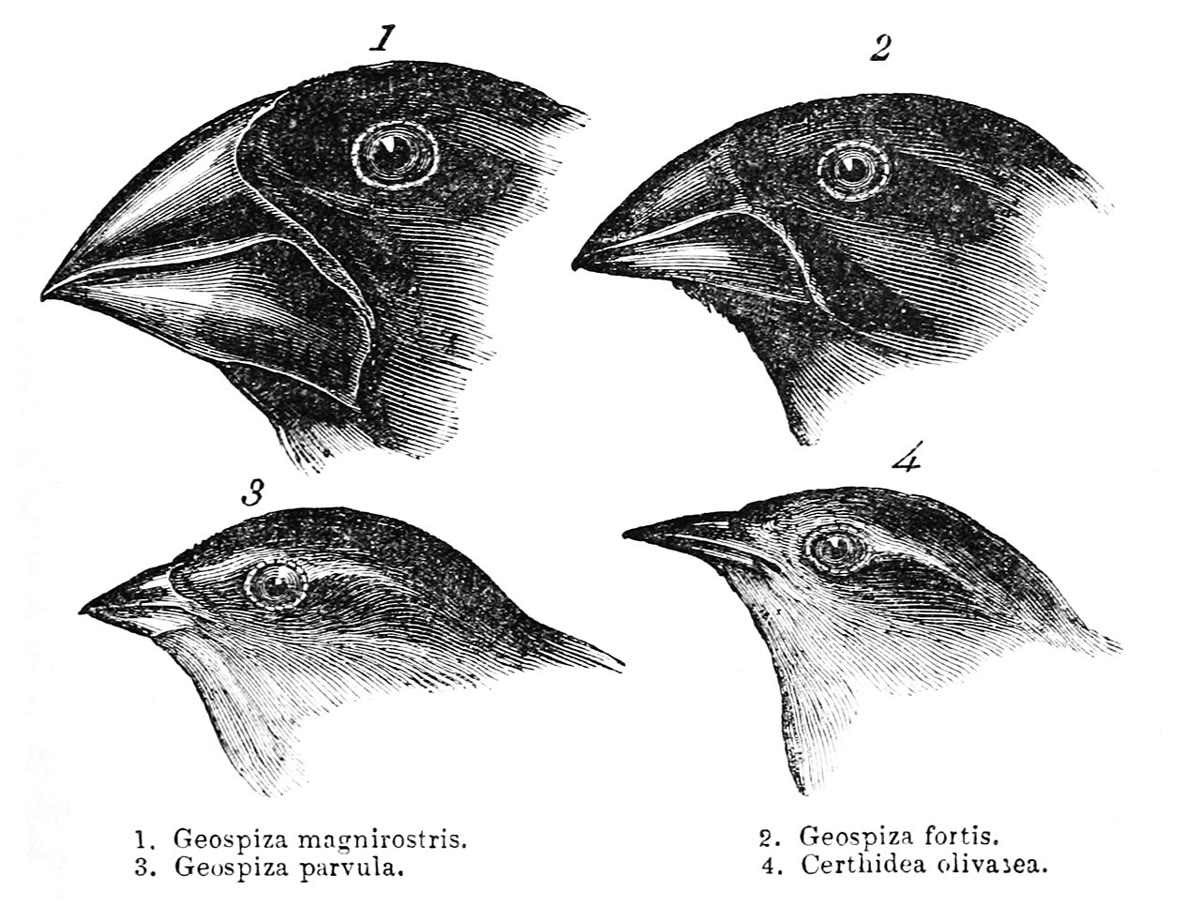
\includegraphics[width=0.44\linewidth]{images/book2/finches-gould.jpg}\hspace{0.04\linewidth}
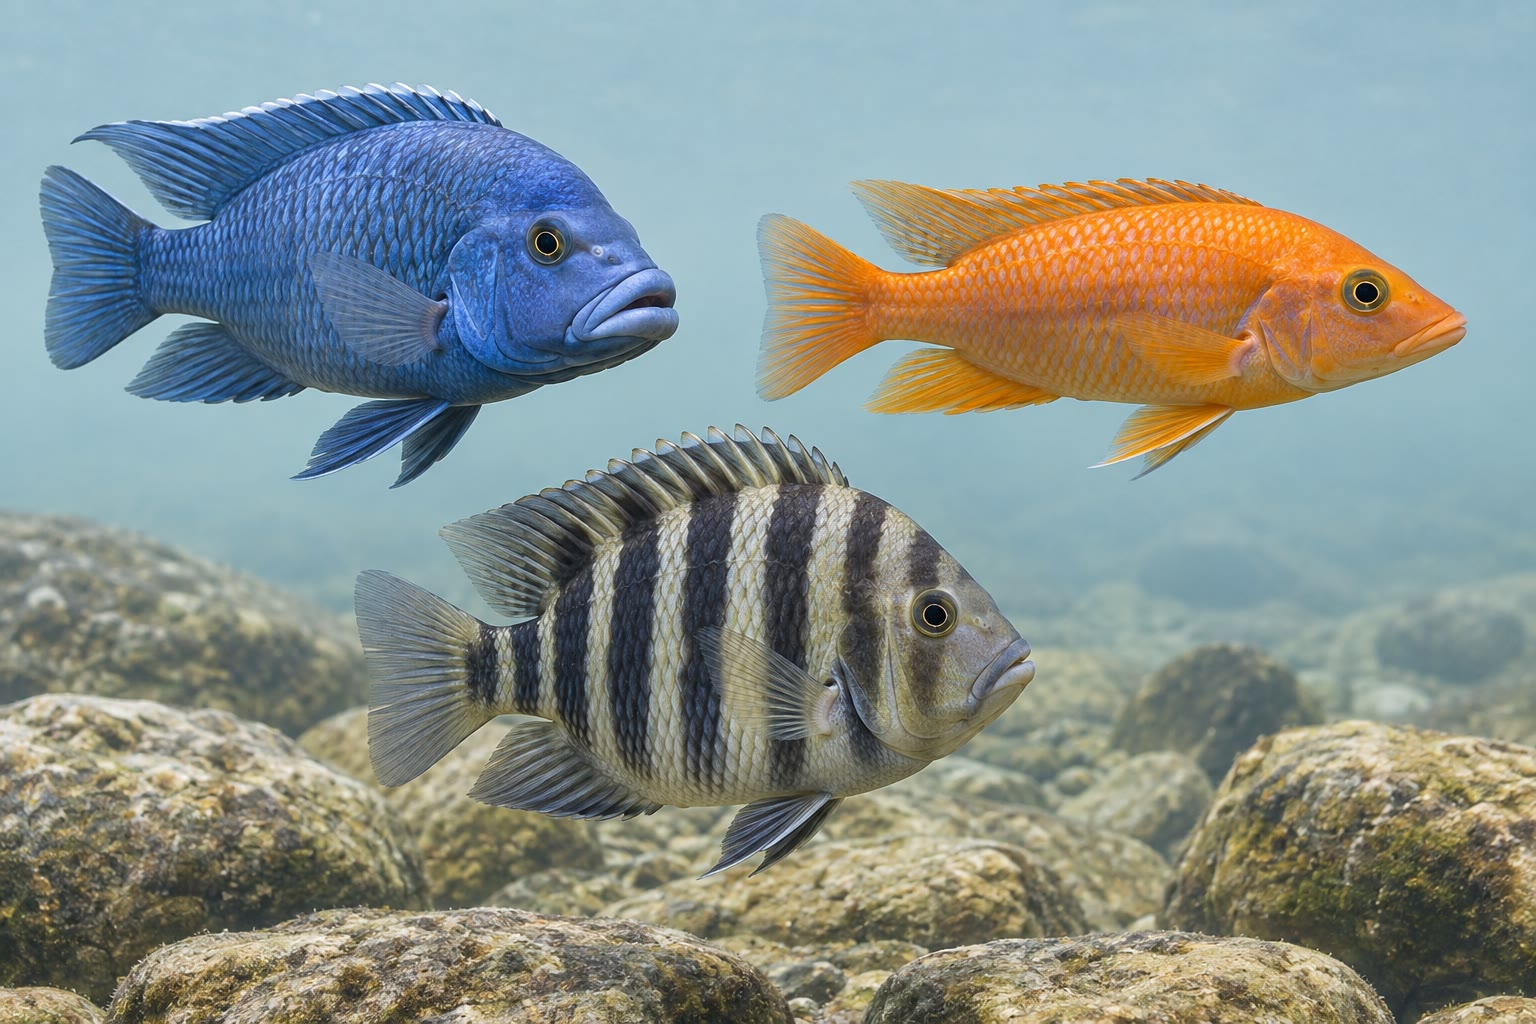
\includegraphics[width=0.44\linewidth]{images/book4/ai/b4-23-cichlids.jpg}

{\small 两次辐射。左：古尔德于 1845 年所绘的达尔文雀，
一个殖民者变成了许多，以喙相区分。
右：非洲湖泊中的慈鲷，由少数奠基者\omterm{def:b2:cell-differentiation:differentiation}{分化}出数百个物种，
各自具有独特的口形与食性。}
\end{omfigure}

\section{大进化：长远视角}

\begin{proposition}[节奏与模式]\label{prop:b2:speciation:tempo}
\index{间断平衡}\index{渐变论}\index{大灭绝}
在几十代之内，蛾改变了体色，雀改变了喙；在数百万年间，
化石记录显示，有些谱系在很长时期内几乎不变，
随后在地质学意义上仅几千年的瞬间，
被一个截然不同的后代所取代——
\emph{\omterm{prop:b2:speciation:tempo}{间断平衡}}，正是小型边缘种群中的\omterm{prop:b2:speciation:modes}{异域物种形成}、
随后扩散，在每十万年取样一次时所呈现的样子；
另有一些谱系，包括马在内，
则在数十个物种之间逐渐变化。
在物种之上，记录呈现的是更替：多数物种存续一百万至一千万年，
\emph{背景灭绝}速率约为每年每百万个物种中灭绝一个，
并曾有五次——奥陶纪末、泥盆纪末、
二叠纪末（其时九成海洋物种消失）、三叠纪末与白垩纪末——
\emph{\omterm{prop:b2:speciation:tempo}{大灭绝}}在数十万年之内清除了当时生存的大部分生物，
重新设定了游戏规则，
幸存者则辐射进入空出的\omterm{prop:b2:speciation:displacement}{生态位}：
在 6600 万年前小行星撞击之后，哺乳动物
进入了恐龙的世界。
大进化是本章与上一章所述微进化
在极长时间内持续推进、并被灾变打断后，
所描绘出的图景。
\end{proposition}

\begin{example}[速率比较]\label{ex:b2:speciation:rates}
在达尔文雀身上，自然选择使喙深在一代之内改变了 \qty{4}{\%}；
整个加拉帕戈斯辐射，即由一个奠基者\omterm{def:b2:cell-differentiation:differentiation}{分化}出的十四个物种，
用了两百万年。小鼠与大象在体型上的差异约为 $10^{5}$ 倍，
若按达尔文雀身上的选择强度计算，仅需几百代即可产生，
但化石记录表明实际用了四千万年。
这一悖论的解决在于注意到：自然选择很少长期朝同一方向作用，
它随环境条件而反转，正如达弗尼大岛在干旱之后的那一年所发生的那样；
而稳定化选择使多数谱系保持在原有位置。
持续的变化十分罕见，这正是物种形成——它恰恰需要持续的变化——
进行得很慢的原因；
也是当世界迅速变化时（正如\cref{ch:b2:global-change}中所述），
无法跟上变化的谱系
便会灭绝。
\end{example}

\section{练习}

\begin{exercise}[$\star$]\label{exo:b2:speciation:1}
叙述\omterm{def:b2:speciation:species}{生物学物种概念}，并给出三种无法应用该概念的情形，
同时说明可代替使用的概念。
\end{exercise}

\begin{exercise}[$\star$]\label{exo:b2:speciation:2}
判别下列情形属于\omterm{prop:b2:speciation:isolation}{合子前隔离}还是\omterm{prop:b2:speciation:isolation}{合子后隔离}：两只青蛙在
不同月份繁殖；骡子；海胆的精子无法与另一物种的卵子结合；
杂交植株生长旺盛，但其\omterm{def:b2:angiosperm-reproduction:seed}{种子}不萌发；
两只蟋蟀的鸣声不同。
\end{exercise}

\begin{exercise}[$\star$]\label{exo:b2:speciation:3}
定义\omterm{prop:b2:speciation:modes}{异域物种形成}、边缘物种形成、\omterm{prop:b2:speciation:modes}{同域物种形成}和\omterm{prop:b2:speciation:modes}{邻域物种形成}，
并各举一例。
\end{exercise}

\begin{exercise}[$\star$]\label{exo:b2:speciation:4}
用文字叙述\omterm{thm:b2:speciation:lv}{洛特卡–沃尔泰拉竞争}的四种结果，
以及稳定共存的条件。
\end{exercise}

\begin{exercise}[$\star\star$]\label{exo:b2:speciation:5}
设 $K_1 = 1000$，$K_2 = 800$，$\alpha = 0.5$，$\beta = 0.6$，
求平衡种群密度，
并验证每个物种都能侵入对方的环境容纳量。
\end{exercise}

\begin{exercise}[$\star\star$]\label{exo:b2:speciation:6}
设 $K_1 = 1000$，$K_2 = 800$，$\alpha = 1.5$，$\beta = 0.3$，
哪一物种获胜？为什么？若 $\alpha = 1.5$ 且 $\beta = 1.5$，结果如何？
\end{exercise}

\begin{exercise}[$\star\star$]\label{exo:b2:speciation:7}
在\omterm{def:b2:meiosis-heredity:meiosis}{二倍体}种群中出现了一个四倍体。求其配子的染色体数，
其与\omterm{def:b2:meiosis-heredity:meiosis}{二倍体}杂交所得后代的染色体数，以及该杂种所产配子的染色体数，
并说明四倍体为何立即被隔离，
为何它仍通常难以延续？
\end{exercise}

\begin{exercise}[$\star\star$]\label{exo:b2:speciation:8}
两个种群自\omterm{def:b2:cell-differentiation:differentiation}{分化}以来各已固定 10 次替换，
两侧新\omterm{def:b2:meiosis-heredity:vocabulary}{等位基因}的每一对互不相容的概率
均为 $0.01$。求当前的期望不相容数，
以及两侧各再固定 30 次替换之后的期望不相容数。
这对隔离与时间的关系有何预测？
\end{exercise}

\begin{exercise}[$\star\star$]\label{exo:b2:speciation:9}
求\omterm{prop:b2:speciation:reinforcement}{杂交带}宽度：每代扩散量 $\sigma =
\qty{2}{km}$、杂种劣势 $s = 0.05$ 时的宽度，以及
在 $\sigma = \qty{0.3}{km}$、$s = 0.4$ 时的宽度。哪一个\omterm{prop:b2:speciation:reinforcement}{杂交带}
更可能以\omterm{prop:b2:speciation:reinforcement}{强化}告终？为什么？
\end{exercise}

\begin{exercise}[$\star\star\star$]\label{exo:b2:speciation:10}
两种雀争夺\omterm{def:b2:angiosperm-reproduction:seed}{种子}，且 $\alpha = \beta = 0.9$，
$K_1 = K_2 = 500$。它们能否共存？\omterm{prop:b2:speciation:displacement}{性状替换}使
$\alpha$ 与 $\beta$ 降至 $0.4$，重新计算平衡状态，
并借助等斜线解释\omterm{prop:b2:speciation:displacement}{性状替换}所起的作用。
\end{exercise}

\begin{exercise}[$\star\star\star$]\label{exo:b2:speciation:11}
格兰特夫妇发现，2004 年干旱后，中地雀的平均喙深
下降了 \qty{0.7}{mm}，$h^{2} = 0.7$，存活者的平均喙深
比种群低 \qty{1}{mm}。
用育种者方程检验这一响应，
并解释决定变化方向的是大地雀的存在，
而非干旱本身。
\end{exercise}

\begin{exercise}[$\star\star\star$]\label{exo:b2:speciation:12}
“物种因偶然而产生，因选择而保留。”试讨论，
结合双位点模型、\omterm{prop:b2:speciation:reinforcement}{强化}作用及地理的作用加以论述。
\end{exercise}

\section{问题：岛上的两种雀}

\begin{problem}[{周末问题——本地雀遭遇入侵者：在相平面上分析二者的竞争，
用育种者方程预测本地雀喙的位移，并以杂交带
衡量二者之间的隔离，
最终给出平衡密度，
喙的位移以及
杂交带宽度}]
\label{pb:b2:speciation:1}
本地物种 1：$K_1 = 1200$，$r_1 = 0.5$（每年）；入侵物种
2：$K_2 = 400$。位移前 $\alpha = 0.9$，$\beta =
0.3$；一次干旱使两者的环境容纳量在一年内都减半。物种 1 的喙
深：均值为 \qty{9.5}{mm}，标准差为
\qty{0.8}{mm}，$h^{2} = 0.7$。\omterm{prop:b2:speciation:reinforcement}{杂交带}参数：$\sigma =
\qty{0.5}{km}$，$s = 0.2$。

\medskip
\noindent\textbf{第一部分——入侵。}
\begin{enumerate}
  \item 写出两条等斜线及其截距。
  \item 能否在 $K_1$ 时入侵物种 1？物种 1
        能否在 $K_2$ 时入侵物种 2？并由此判断结局。
  \item 求平衡密度。
  \item 计算物种 2 到达时的 $\mathrm{d}N_1/\mathrm{d}t$，
        其中 $N_2 = 20$，$N_1 = 1200$。其符号
        说明什么？
  \item 干旱期间两个 $K$ 均减半，重新计算
        平衡状态，并说明两物种的数量各发生怎样的变化。
  \item 为什么入侵者对本地种的影响（$\alpha = 0.9$）
        大于本地种对入侵者的影响（$\beta = 0.3$）？
\end{enumerate}

\medskip
\noindent\textbf{第二部分——\omterm{prop:b2:speciation:displacement}{性状替换}。}
干旱期间，喙最大的本地种个体与入侵者竞争最为激烈，
并因此死亡：存活者的平均
喙深为 \qty{9.0}{mm}。
\begin{enumerate}[resume]
  \item 计算选择差和响应。
  \item 给出下一代的平均喙深。
  \item \omterm{prop:b2:speciation:displacement}{性状替换}之后，$\alpha$ 降至 $0.5$，重新计算
        平衡状态（$K$ 取原值）。
  \item 解释\omterm{prop:b2:speciation:displacement}{性状替换}对物种 1 的等斜线产生了什么影响。
  \item 若这一强度的选择每年都作用，
        需要多少年才能使喙深改变 \qty{2}{mm}？为何
        实际上并非如此？
  \item 将其与该适应辐射的两百万年
        历史相比较，并加以评述。
\end{enumerate}

\medskip
\noindent\textbf{第三部分——隔离。}
两个物种可以杂交；杂种的喙为中间型，
\omterm{def:b2:population-genetics:fitness}{适合度}为 $1 - s$。
\begin{enumerate}[resume]
  \item 指出在达尔文地雀中使杂交罕见的
        \omterm{prop:b2:speciation:isolation}{合子前隔离}机制，以及杂种的一种
        合子后代价。
  \item 计算两者之间\omterm{prop:b2:speciation:reinforcement}{杂交带}的宽度，取 $\sigma
        = \qty{0.5}{km}$，$s = 0.2$。
  \item 岛屿宽 \qty{1}{km}。这说明什么？
  \item 解释\omterm{prop:b2:speciation:reinforcement}{强化}作用将如何进行，
        以及它将作用于何种性状。
  \item 本地种的两个种群分别位于不同岛屿，
        自分开以来各自固定了 15 个替换；
        任一配对不相容的概率为 $0.005$。计算期望的
        不相容配对数，并判断两者是否为不同物种。
  \item \omterm{def:b2:speciation:species}{生物学物种概念}、形态学\omterm{def:b2:speciation:species}{物种概念}与
        系统发生\omterm{def:b2:speciation:species}{物种概念}，对两个岛屿种群的判断是否一致？
        请加以解释。
\end{enumerate}

\medskip
\noindent\textbf{第四部分——长远视角。}
\begin{enumerate}[resume]
  \item 若一个物种平均存续 500 万年，其
        背景灭绝率（每物种每年）为多少？对于含 1000 万个物种的
        生物区系，每年有多少次灭绝？
  \item 当前灭绝速率估计为背景速率的 100 至 1000
        倍。这相当于每年灭绝多少个物种？
  \item 一次大规模灭绝使 \qty{75}{\%} 的物种
        在 \num{100000} 年内消失，将其速率与当前速率相比较。
  \item 用一句话解释大规模灭绝的幸存者
        为何会发生适应辐射。
  \item 化石记录中的一个谱系在 300 万年间变化很小，
        随后在 \num{20000} 年内被一个不同的
        后代所取代。指出该模式，并给出产生它的
        物种形成方式。
  \item 以雀类每代 \qty{4}{\%} 的变化速率为依据，需要多少代
        持续选择才能使喙深加倍？为何化石记录显示
        此类变化需要数百万
        年？
  \item 概括结果：\omterm{prop:b2:speciation:displacement}{性状替换}前后的竞争结局与平衡状态，
        一代内的喙位移，以及
        \omterm{prop:b2:speciation:reinforcement}{杂交带}宽度。
\end{enumerate}
\end{problem}
